\documentclass{article}


% if you need to pass options to natbib, use, e.g.:
%     \PassOptionsToPackage{numbers, compress}{natbib}
% before loading neurips_2023


% ready for submission
\usepackage[final]{neurips_2023}


% to compile a preprint version, e.g., for submission to arXiv, add add the
% [preprint] option:
%     \usepackage[preprint]{neurips_2023}


% to compile a camera-ready version, add the [final] option, e.g.:
%     \usepackage[final]{neurips_2023}


% to avoid loading the natbib package, add option nonatbib:
%    \usepackage[nonatbib]{neurips_2023}


\usepackage[utf8]{inputenc} % allow utf-8 input
\usepackage[T1]{fontenc}    % use 8-bit T1 fonts
\usepackage{hyperref}       % hyperlinks
\usepackage{url}            % simple URL typesetting
\usepackage{booktabs}       % professional-quality tables
\usepackage{amsfonts}       % blackboard math symbols
\usepackage{nicefrac}       % compact symbols for 1/2, etc.
\usepackage{microtype}      % microtypography
\usepackage{xcolor}         % colors
\usepackage{graphicx}
\usepackage{amsmath}
\usepackage{listings}

\lstset{basicstyle=\ttfamily,
  showstringspaces=false,
  commentstyle=\color{red},
  keywordstyle=\color{blue}
}

\title{Realtime Object-Detection In Gaming: Fine-Tuning for Valorant}


% The \author macro works with any number of authors. There are two commands
% used to separate the names and addresses of multiple authors: \And and \AND.
%
% Using \And between authors leaves it to LaTeX to determine where to break the
% lines. Using \AND forces a line break at that point. So, if LaTeX puts 3 of 4
% authors names on the first line, and the last on the second line, try using
% \AND instead of \And before the third author name.


\author{
  Liu Chang \thanks{
    Group Leader, pipeline implementation, model training, presenter, and paper writer.
  }\\
  ShanghaiTech University\\
  \texttt{liuchang2023@shanghaitech.edu.cn} \\
  \And
  Liu Changyu \thanks{
    Model training, fine-tuning, and evaluation.
  }\\
  ShanghaiTech University\\
  \texttt{liuchy2023@shanghaitech.edu.cn} \\
  \And
  Qiu Zhaolin\\
  ShanghaiTech University\\
  \texttt{qiuzhl2023@shanghaitech.edu.cn} \\
}


\begin{document}


\maketitle


\begin{abstract}

\end{abstract}


\section{Introduction}


The confluence of deep learning and interactive entertainment has catalyzed a paradigm shift, unlocking possibilities that were once the domain of science fiction. Video games, now a dominant global cultural and economic force, represent a uniquely challenging and fertile ground for the application of real-time computer vision. The ability to perceive, understand, and react to dynamic, visually complex game environments in milliseconds is a cornerstone of human play. Replicating this capability with artificial intelligence opens a dual-edged sword: it presents an unprecedented threat to competitive integrity while simultaneously offering powerful new tools for accessibility and intelligent agent design.

A significant and pressing challenge emerging from this technological advancement is the rise of vision-based cheating in competitive games, particularly in the First-Person Shooter (FPS) genre. Traditionally, cheating involved direct memory injection or network packet manipulation—methods that could be reliably identified by anti-cheat software scanning for unauthorized code and memory access. However, modern vision-based cheats operate on a fundamentally different principle. By capturing the game's video output—the same visual information a human player sees—and processing it with a convolutional neural network (CNN), these systems can identify and aim at opponents with superhuman precision. Because they interface with the game solely through screen capture and simulated mouse/keyboard inputs, they mimic legitimate human interaction, rendering them exceptionally difficult to detect with conventional anti-cheat mechanisms. This new class of "AI aimbots" poses a profound threat to the fairness and long-term viability of the multi-billion dollar esports and competitive gaming industry.

Conversely, the very same technology holds immense promise for positive transformation. Vision AI is proving to be a powerful enabler of game accessibility, helping to break down barriers for players with disabilities. A recent, award-winning example is the work by NetEase, which utilized vision AI to provide real-time screen narration and touch-based assistance, making complex game interfaces accessible to visually impaired players \cite{neteaseAIEyes2024}. This application highlights a path where real-time object and UI element detection can be harnessed to create more inclusive gaming experiences, from automated highlighting of critical game objects to providing auditory cues for environmental threats.

Furthermore, the integration of vision is poised to revolutionize the design of in-game Non-Player Characters (NPCs). For decades, game AI has been largely dependent on brittle and predictable systems like behavior trees and finite state machines, which often rely on privileged access to the game engine's internal state. This leads to enemy behaviors that, while functional, lack the adaptability and emergent complexity of human opponents. In contrast, an AI agent that perceives the game world through vision—akin to a human player—can be trained via reinforcement learning (RL) to develop sophisticated, human-like strategies. Seminal work in complex games like StarCraft II, often driven by the player community, has demonstrated that visually-grounded RL agents can achieve grandmaster-level performance, showcasing a future where NPCs can provide more engaging, challenging, and realistic interactions \cite{vinyals2017starcraft,li2024multiagent}.

Despite this clear duality, a systematic and public investigation into the practical performance of modern object detection models within the real-time constraints of a live game environment is lacking. The core challenge is multifaceted: any viable system, whether for nefarious or beneficial purposes, must achieve high accuracy while maintaining minimal inference latency and a low computational footprint to avoid disrupting the game's performance. This necessitates a move beyond general-purpose benchmarks to a specific analysis of lightweight, efficient architectures operating under the unique visual conditions and temporal demands of gaming.

This paper aims to bridge this gap. We present a comprehensive study focused on implementing and evaluating a real-time object detection pipeline for video games. Our work is guided by the need to understand the capabilities of vision-based exploits while simultaneously laying the groundwork for positive innovation. Our primary contributions are as follows:

\begin{itemize}
\item[1.] \textbf{Feasibility Analysis of Vision-Based Cheating}: We develop and empirically evaluate a real-time object detection pipeline tailored for FPS games. By fine-tuning and deploying this system, we provide a quantitative baseline for the performance and viability of vision-based automated targeting, offering crucial data for the anti-cheat research community.

\item[2.] \textbf{Benchmarking for Real-Time Performance}: We conduct a comparative analysis of several state-of-the-art, lightweight object detection architectures (e.g., YOLOv8, FastSAM, RT-DETR). We systematically benchmark their performance on custom-annotated game footage, focusing on the critical trade-offs between mean Average Precision (mAP), inference speed (FPS), and resource utilization on consumer-grade hardware.

\item[3.] \textbf{A Foundation for Positive Applications}: We detail a streamlined methodology for data collection, annotation, and model fine-tuning. The resulting models and robust pipeline serve as a valuable reference and an open-source foundation for researchers and developers aiming to build assistive technologies for accessibility or to create the next generation of intelligent, vision-driven RL agents.
Through this work, we provide a foundational study on the practical application of computer vision in modern gaming, addressing its most immediate challenges and illuminating its most promising opportunities.
\end{itemize}

\section{Related Work}
\subsection{Object Detection and Segmentation Models}

\paragraph{YOLOv8} \cite{reis2024realtimeflyingobjectdetection} is one of the most popular object detection models of the YOLO (You Only Look Once) family, known for its speed and accuracy. It employs a single-stage architecture that predicts bounding boxes and class probabilities directly from full images in one evaluation, making it suitable for real-time applications. YOLOv8 introduces several improvements over its predecessors, including better feature extraction through CSPNet, enhanced anchor-free detection, and improved training techniques that allow it to achieve high mAP while maintaining low inference latency.

\paragraph{FastSAM} \cite{zhao2023fast} is a lightweight segmentation model designed for real-time applications. It builds upon the principles of SAM (Segment Anything Model) but optimizes for speed and efficiency, making it suitable for scenarios where computational resources are limited. FastSAM uses a simplified architecture that reduces the number of parameters and computational overhead while maintaining competitive segmentation performance. Its design allows for quick inference times, making it ideal for applications requiring rapid object detection and segmentation.

\paragraph{RT-DETR} \cite{lv2023detrs} (Real-Time DEtection TRansformer) is a real-time object detection model that adapts the DETR (DEtection TRansformer) architecture for faster inference. DETR revolutionized object detection by treating it as a direct set prediction problem, using transformers to model relationships between objects in an image. RT-DETR modifies this approach to improve speed, making it feasible for real-time applications. It achieves this by optimizing the transformer architecture and reducing the computational complexity, allowing for efficient processing of images while maintaining high accuracy.


\subsection{Anti-Cheat Methods}

\paragraph{Traditional Anti-Cheat Methods} There are three main categories of traditional anti-cheat methods: player client detection, game network communication detection, and game remote server detection. However, these methods are often limited by the need for privileged access to the game client or server, making them ineffective against vision-based cheats that operate solely through screen capture and simulated inputs.

\paragraph{Deep Learning for Anti-Cheat} To combat vision-based cheats, researchers have explored the use of deep learning techniques for cheat detection. For instance, Spijkerman and Marie Ehlers \cite{10.1145/3440840.3440857} applied Support Vector Machines (SVMs), decision trees, and Naive Bayes machine learning models to analyze players' mouse and keyboard operations. By integrating learning features into SVM models, they achieved superior cheating detection results. However, relying solely on SVMs for cheating detection may overlook crucial information such as players' aiming frequency, hit rates, and pre-aim positions.

\section{Method}
\label{method}

\subsection{Data Collection and Annotation}

We collected a dataset of game \textit{Valorant} from Santyasa dataset from Roboflow \cite{santyasa_roboflow}, which contains 3771 images of various game scenes and annotations of enemy heads and bodies. The annotations are in the form of bounding boxes, which fit the COCO format. The dataset is split into training, validation, and test sets, with 80\% for training, 10\% for validation, and 10\% for testing.

Also, we collected a corner case dataset of 100 images from gaming records, where the players are at tricky angles or positions, such as the edge of the screen, behind obstacles or inside a smoke grenade. This dataset is used to test the robustness of the model in real-time scenarios.

\subsection{Training}

As mentioned, we will fine-tune three different object detection models: YOLOv8, FastSAM, and RT-DETR. The training process involves the following steps:

\paragraph{Loading the Dataset and Models} We load the training and validation datasets using our custom dataset loader. Then we load the pre-trained weights of the models we want to fine-tune. The pre-trained weights are obtained from the ultralytics repository.

\paragraph{Training with Parameters} We adjust the training parameters such as learning rate, batch size, number of epochs, and optimizer. The learning rate is set to 0.01, the batch size is set to 16, and the number of epochs is set to 100. We use the Auto Optimizer from the ultralytics repository, which automatically selects the best optimizer for the model. The training results can be seen in Section \ref{appendix}.

\paragraph{Loss Function} The default loss function for YOLOv8 is
$$
\mathcal{L}_{YOLO} = \alpha_{box}\mathcal{L}_{box} + \alpha_{cls}\mathcal{L}_{cls} + \alpha_{dfl}\mathcal{L}_{dfl} 
$$
where $\mathcal{L}_{box}$ is the bounding box regression loss, $\mathcal{L}_{cls}$ is the classification loss, and $\mathcal{L}_{dfl}$ is the distribution focal loss. The hyperparameters $\alpha_{box}$, $\alpha_{cls}$, and $\alpha_{dfl}$ are set to 9.0, 0.3, and 1.8 respectively.

\subsection{Model Fine-Tuning}

\paragraph{Transfer Learning with Frozen Layers} We apply transfer learning by freezing the initial layers of the models and only training the last few layers. This allows us to leverage the pre-trained weights while adapting the models to our specific dataset. The frozen layers are determined based on the model architectures. For YOLOv8, we freeze the first 10 backbone and feature extract layers, while for FastSAM and RT-DETR, we freeze the first 5 backbone layers. This helps to retain the general features learned from the pre-trained models while fine-tuning them with a faster convergence.


\begin{figure}[htbp]
  \centering
  \begin{minipage}{0.5\textwidth}
    \centering
    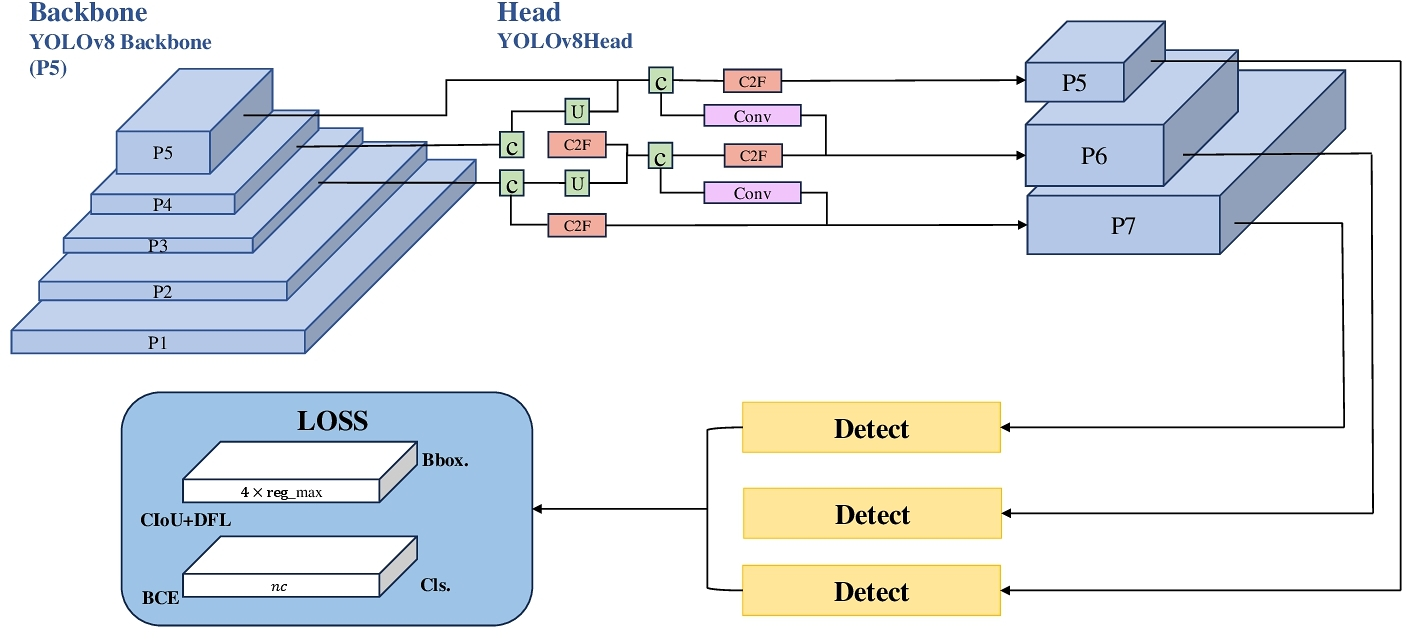
\includegraphics[width=\linewidth]{images/yolo-arch.jpg}
    \caption{Architecture of YOLOv8. We freeze the backbone layers only.}
    \label{fig:yolo-arch}
  \end{minipage}%
  \hfill
  \begin{minipage}{0.5\textwidth}
    \centering
    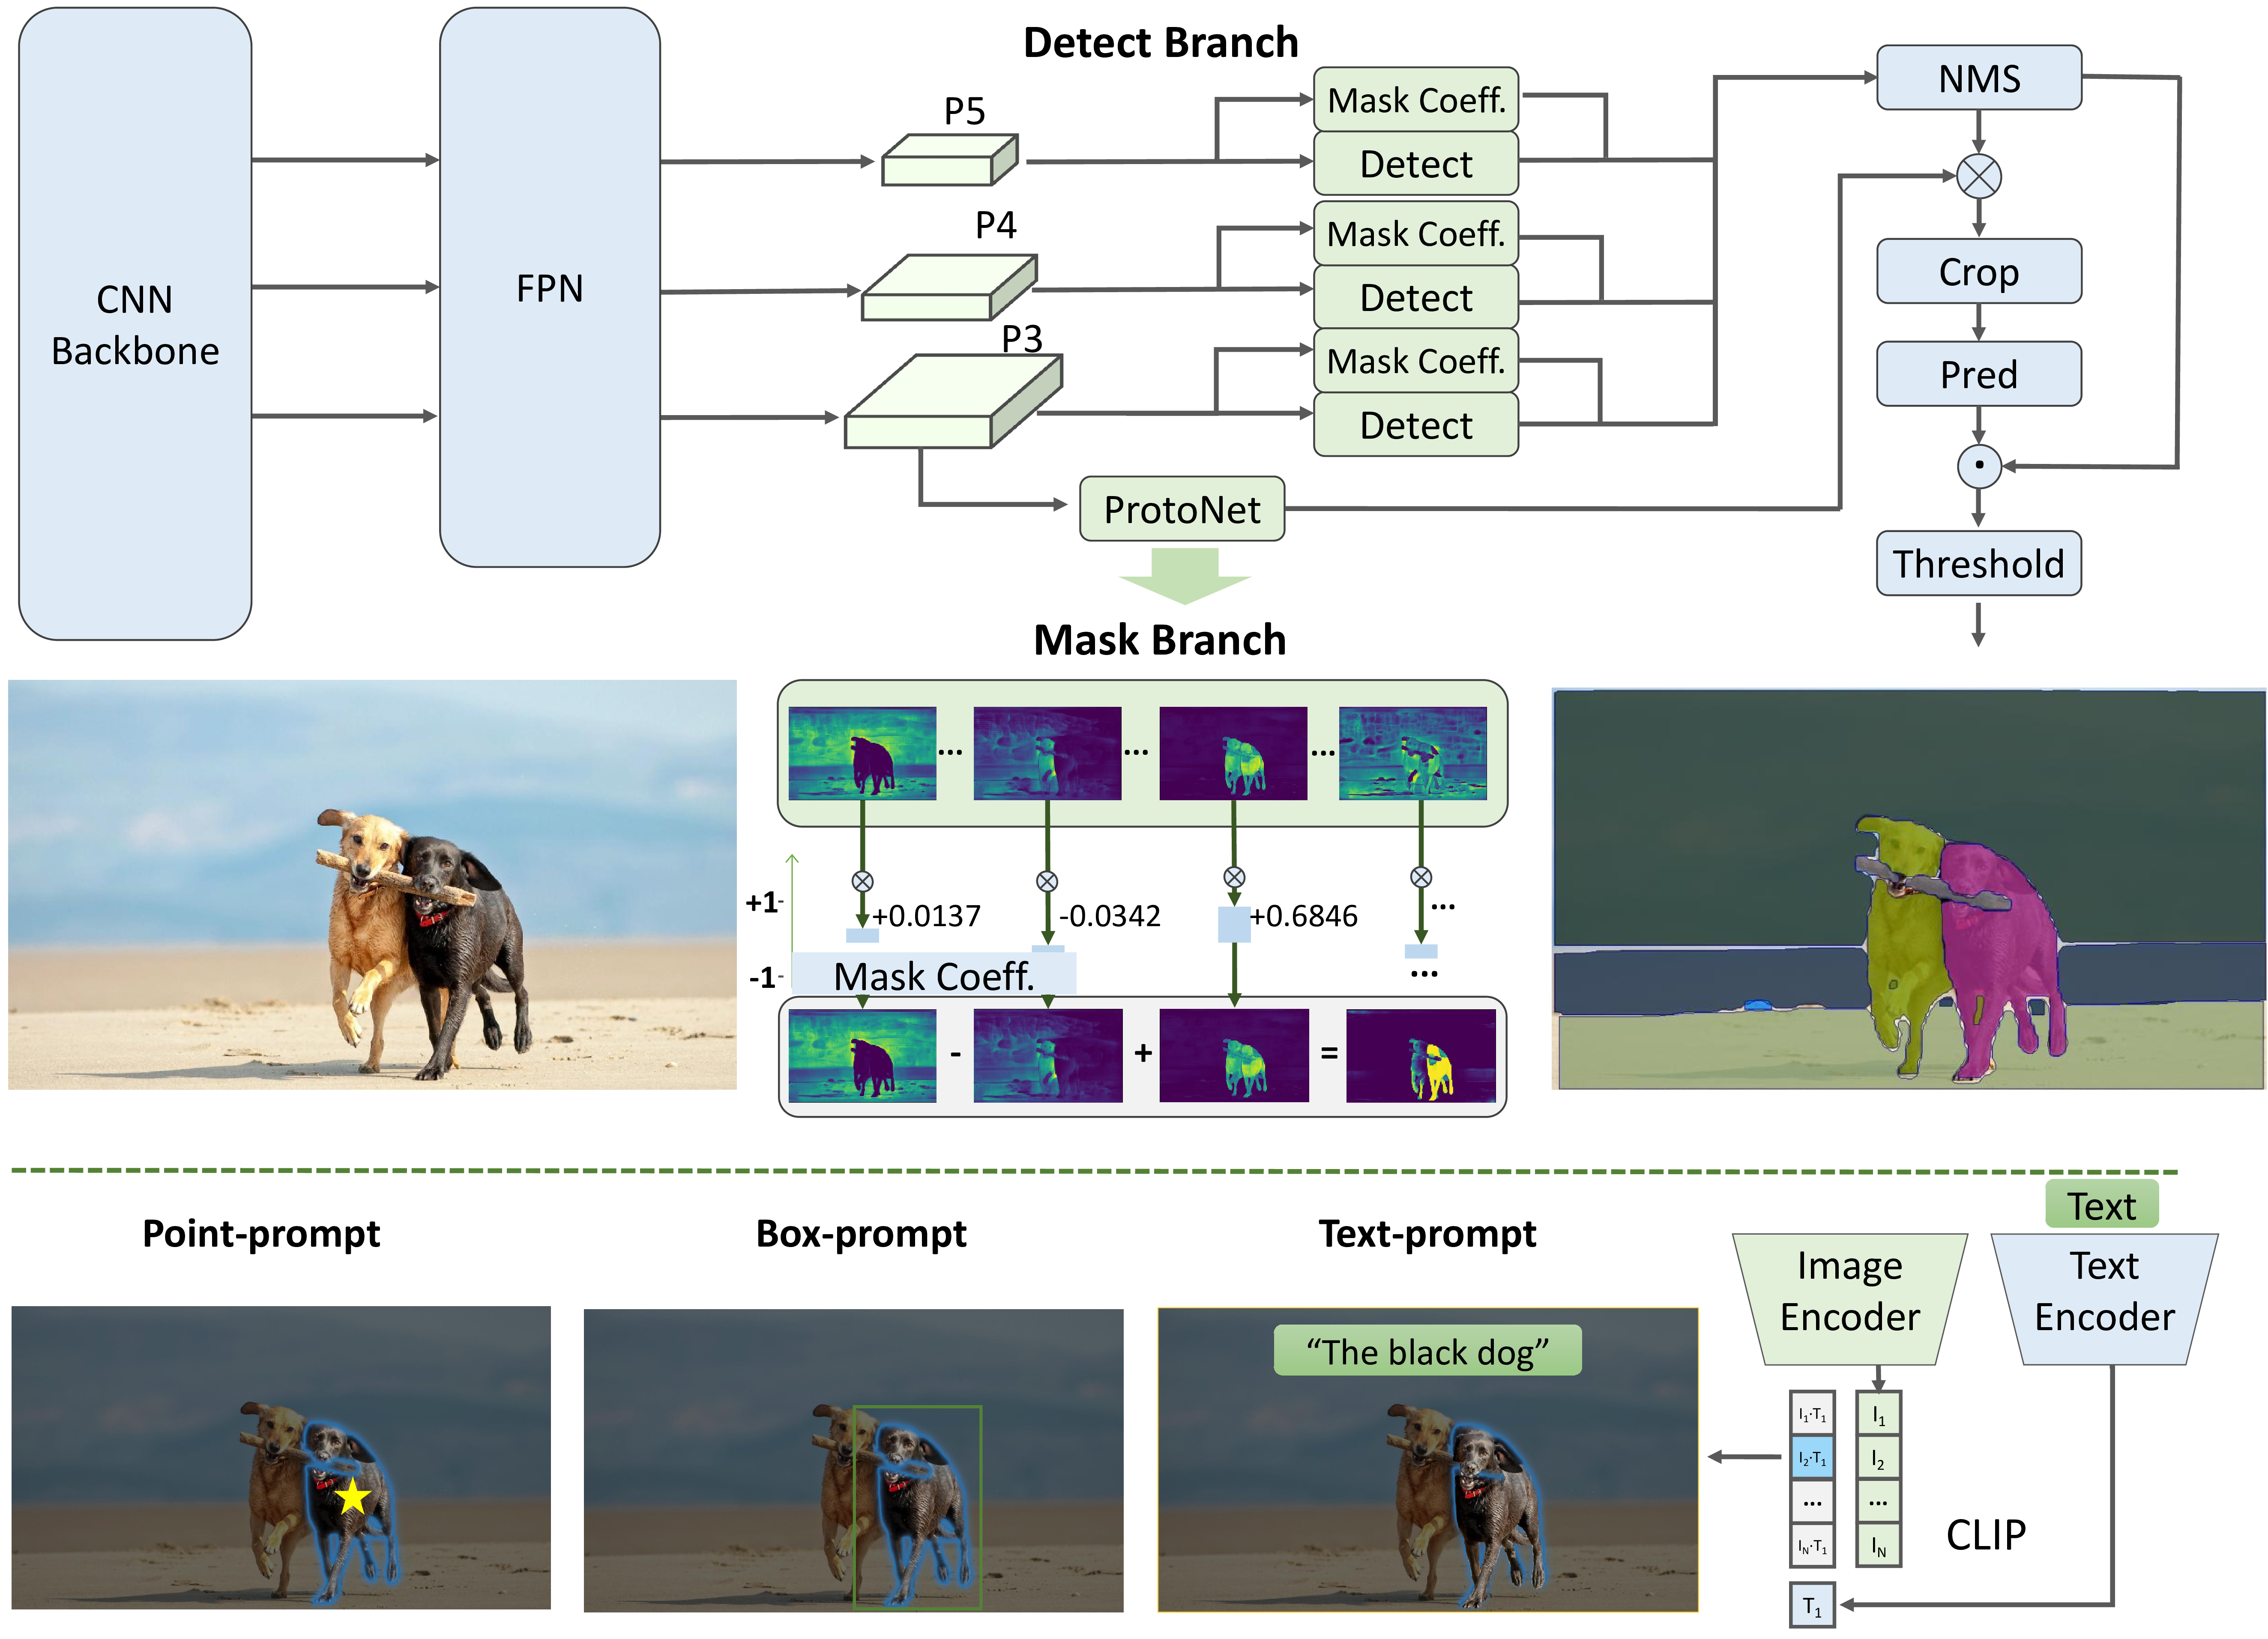
\includegraphics[width=\linewidth]{images/fastsam-arch.png}
    \caption{Architecture of FastSAM. We freeze the backbone layers only.}
    \label{fig:fastsam-arch}
  \end{minipage}%

  \begin{minipage}{0.8\textwidth}
    \centering
    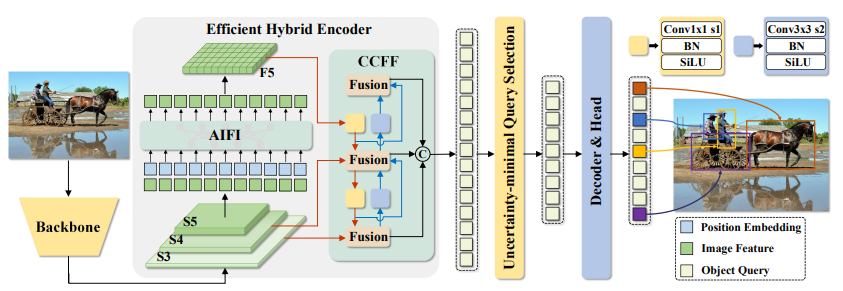
\includegraphics[width=\linewidth]{images/rtdetr-arch.png}
    \caption{Architecture of RT-DETR. We freeze the backbone layers only.}
    \label{fig:rt-detr-arch}
  \end{minipage}
  \caption{Three images arranged horizontally.}
  \label{fig:three_horizontal_images}
\end{figure}

\subsection{Dataset Augmentation}
To enhance the robustness of our models, we apply various data augmentation techniques during training. These include:
\begin{itemize}
\item \textbf{Random Rotation}: Randomly rotating the images in $[-15^{\circ}, 15^{\circ}]$ to simulate different viewing angles.
\item \textbf{Noise}: Adding random Gaussian noise to the images to simulate different lighting conditions and camera quality.
\item \textbf{Brightness and Contrast Adjustment}: Randomly adjusting the brightness and contrast of the images in $[0.85, 1.15]$ range to simulate different lighting conditions.
\end{itemize}
Therefore, the total number of training images is increased to $5934$.

\subsection{Model Evaluation}

The metrics used to evaluate the performance of the models are:
\begin{itemize}
  \item \textbf{Precision}:   This metric measures the accuracy of the model: 
  $$
  \text{Precision} = \frac{TP}{TP + FP}
  $$
  where $TP$ is the number of true positives (correctly detected objects), and $FP$ is the number of false positives (incorrectly detected objects). 
  \item \textbf{Recall}: This metric measures the ability of the model to find all the relevant objects. The way to calculate recall is
  $$
  \text{Recall} = \frac{TP}{TP + FN}
  $$
  where $FN$ is the number of false negatives (missed objects). Recall indicates how many of the relevant objects were actually detected.
  \item \textbf{F1 Score}: This metric combines precision and recall into a single score. The way to calculate F1 score is
  $$
  \text{F1 Score} = 2 \cdot \frac{\text{Precision} \cdot \text{Recall}}{\text{Precision} + \text{Recall}}
  $$
  The F1 Score provides a balance between precision and recall, especially when the class distribution is imbalanced.
  \item \textbf{Mean Average Precision (mAP)}: This metric measures the accuracy of the model in detecting objects. It is calculated as the average precision across all classes, taking into account both precision and recall.
\end{itemize}

\subsection{Real-Time Inference Pipeline}

\paragraph{Different Input Sources} The pipeline supports different input sources, including video files, images, and live window capture. Use the command argument '--input\_method' to specify the input source. 

\paragraph{Different Model Types} The pipeline supports different model types, including YOLOv8, FastSAM, and RT-DETR. Use the command argument '--model\_type' to specify the model type.

\paragraph{Prune} The pipeline allows for pruning the model to reduce its size and improve inference speed. Using command argument '--prune\_percent=0.3' will prune 30\% of the model's parameters.

\paragraph{Results} See results in Section \ref{appendix}

\section{Experiments}
\label{experiments}

\subsection{Experimental Equipment}

The experiments were conducted both on a cluster of NVIDIA 3090 GPUs and on a PC with a NVIDIA RTX 4090 GPU. 

\subsection{Tests and Results}

We conducted a series of tests to evaluate the performance of the models from their baseline to the fine-tuned version. The tests were conducted on the same dataset, and the results are shown in Table \ref{tab:model_performance}. The $^*$ indicates the frozen layers of the model. 

\begin{table}[htbp]
  \centering
  \begin{tabular}{c|c|c|c|c|c|c|c|c}
    \hline
    Model & Epochs & Train Time(s) & \#Params & Precision & Recall & F1-score & AP$^{50}$ & AP$^{50-95}$ \\
    \hline
    YOLOv8 & 0 & 0 & 6.9M & 0.001 & 0.041 & 0.0019 & 0.0004 & 0 \\
    YOLOv8 & 100 &  & 6.9M &  &  &  &  &  \\
    YOLOv8$^*$ & 100 & 8904.2 & 6.9M & 0.7664 & 0.5825 & 0.6706 & 0.6478 & 0.3160 \\
    FastSAM & 0 & 0 & 72.2M & 0.0002 & 0.052 & 0.0004 & 0.0001 & 0\\
    FastSAM & 100 & 8750.78 & 72.2M & 0.7799 & 0.7991 & 0.7894 & 0.8620 & 0.4112 \\
    FastSAM$^*$ & 100 & 8050.18 & 72.2M & 0.8667 & 0.5657 & 0.6846 & 0.8548 & 0.3950 \\
    RT-DETR & 0 & 0 & 45M & 0.173 & 0.168 & 0.171 & 0.095 & 0.046 \\
    RT-DETR & 100 & 10284.6 & 45M & 0.619 & 0.483 & 0.543 & 0.465 & 0.1829 \\
    RT-DETR$^*$ & 100 & 9700.3 & 45M & 0.667 & 0.360 & 0.467 & 0.375 & 0.170 \\
    \hline
  \end{tabular}
  \caption{Performance comparison of different models.}
  \label{tab:model_performance}
\end{table}

Then we add our corner case dataset to the training set and fine-tune the original models with the same parameters again. We evaluate the performance on the corner case test set, and compairing with the best models shown in the Table \ref{tab:model_performance} above, we can see that the performance of the models trained on mixed dataset is significantly improved. The results are shown in Table \ref{tab:corner_case_performance}. The $^*$ indicates the models are trained with the corner case dataset.

\begin{table}[htbp]
  \centering
  \begin{tabular}{c|c|c|c|c|c|c}
    \hline
    Model & Epochs & Precision & Recall & F1-score & AP$^{50}$ & AP$^{50-95}$ \\
    \hline
    YOLOv8 & 100 &  &  &  &  &  \\
    YOLOv8$^*$ & 100  &  &  &  &  &  \\
    FastSAM & 100  & 0.011  & 0.030 & 0.016 & 0.0071 & 0.0036 \\
    FastSAM$^*$ & 100  & 0.829 & 0.451 & 0.584 & 0.497 & 0.206 \\
    RT-DETR & 100  & 0.0005 & 0.0627 & 9.99e-04 & 0.0004 & 5.29e-05 \\
    RT-DETR$^*$ & 100  & 0.552 & 0.539 & 0.545 & 0.476 & 0.253 \\
    \hline
  \end{tabular}
  \caption{Performance comparison of different models.}
  \label{tab:corner_case_performance}
\end{table}

\section{Conclusion}
\label{conclusion}



\section{Appendix}
\label{appendix}

\subsection{Training Results}


{
\small

\bibliographystyle{unsrt}
\bibliography{reference}
}

%%%%%%%%%%%%%%%%%%%%%%%%%%%%%%%%%%%%%%%%%%%%%%%%%%%%%%%%%%%%


\end{document}
